\documentclass[../notes.tex]{subfiles}

\pagestyle{main}
\renewcommand{\chaptermark}[1]{\markboth{\chaptername\ \thechapter\ (#1)}{}}

\begin{document}




\chapter{Review and Intro to NMR}
\section{Introduction and Review}
\begin{itemize}
    \item \marginnote{1/11:}We're skipping alcohols and ethers and coming back later because that's what third quarter really focuses on.
    \item What you need to worry about is class content --- if he doesn't mention it, even if it's in the book, we won't be responsible for it on exams.
    \item Natural products inspire new drugs.
    \begin{itemize}
        \item Salicylic acid mediates pain, but it will erode the lining of your stomach.
        \item Hoffmann functionalizes the alcohol to an ester, removing the negative effects and creating aspirin.
    \end{itemize}
    \item Sucrose (table sugar) is glucose plus fructose. Glucose tastes slightly less sweet, and fructose tastes a whole lot sweeter.
    \item We now consume 120 pounds of sugar per person per year, different from 20 pounds per person per year in 1976 and 1 pound per person per year in older times.
    \begin{itemize}
        \item So we have developed artificial sweeteners that cut calories, such as saccharin, aspartame, and sucralose.
        \item Sucralose is thermally stable (you can bake with it), has no chloric content, and is made from sugar by protecting some alcohols and replacing others with chlorines.
    \end{itemize}
    \item Capsaicin (spiciness) evolved to prevent bugs from biting their host plants.
    \begin{itemize}
        \item Both capsaicin and resiniferatoxin have the same vanillin group; thus, this group is probably important for reacting with pain receptors.
    \end{itemize}
    \item Compactin from mushrooms lowers cholesterol.
    \begin{itemize}
        \item Zocor and lipitol are derived from it!
    \end{itemize}
    \item Taxol (breast cancer treatment) accumulates slowly in rare trees.
    \begin{itemize}
        \item We can derive from the needles (a renewable resource), however, a compound that is easily functionalized to taxol.
    \end{itemize}
    \item It is essential to understand the mechanisms in this course!
    \begin{itemize}
        \item We won't have to worry much about competing reactivity, but we do need to know how reactivity can change in different situations.
    \end{itemize}
    \item Quinine treats malaria.
    \begin{itemize}
        \item Quinine is what makes fizzy water taste bitter.
        \item In trying to fabricate Quinine, Perkin discovers a compound that dyes fabric purple. Never gets his PhD but makes millions off of this invention. Before, only royals could wear purple (the sole source was mediterranean sea slugs).
    \end{itemize}
    \item Identify S\textsubscript{N}1 by the fact that all chiral information in the reactant will be lost.
    \item Identify S\textsubscript{N}2 by the inversion of stereochemistry.
    \item We won't worry much about E1 this quarter.
    \item We'll see a lot of E2 this quarter.
    \item We'll look into radical and pericyclic (Diels-Alder) reactions this quarter.
    \item Molecules that may look similar can actually be quite different.
    \item Color is related to the number of double bonds in a molecule.
    \item Blue lobsters are blue because they have enough of an enzyme to sequester all of the colorant in the shells of the lobsters.
    \begin{itemize}
        \item Would you pay more for it because of its rare color? Probably shouldn't because cooking it will still make it red. It won't taste any better.
    \end{itemize}
    \item Fleming and penicillin.
    \begin{itemize}
        \item Initially we have no idea what its structure is.
        \item It's hard to synthesize something if we have no idea what it is.
        \item During WWII, American and Britain embark on a campaign to synthesize penicillin equal in scope to the Manhatten project, but it wasn't successful.
        \item Eventually, Dorthy Crowfoot Hodgkin gets its structure with x-ray crystallography, after wrong attempts from R. B. Woodward and Sir Robert Robinson (future Nobel laureates who hated each other).
        \item The moldy cantaloupe.
        \item In 1955, John Sheehan at MIT comes up with the first chemical reagent capable of synthesizing penicillin's 4-membered ring.
        \item But we made too many antibiotics and antibiotic resistance developed.
        \item MRSA is only killed by vancomycin, but they're even developing resistance to that.
        \item Thinking chemically to get off the pesticide treadmill.
        \item We need the sophistication of nature to build molecules more complex than we can build en masse pharmaceutically.
        \item As species go extinct, though, we are losing potential weapons.
    \end{itemize}
    \item X-ray crystallography pinpoints the location of all atoms other than hydrogen in a molecule.
    \item Line-angle is gonna be big this quarter.
    \item We will not be tested on IUPAC nomenclature, but we should know it just to be able to communicate.
    \item Talks about resonance and induction.
    \item The IR spectroscopic signal of a carbonyl is $\SI{1700}{\per\centi\meter}$.
    \item Resonance affects acidity and IR spectroscopy --- bonds that resonate (have less double bond character) will have lower IR frequencies.
    \item A lot of reactions are quenched by an \ce{H3O+} workup --- just enough to quench, not enough to react.
\end{itemize}



\section{Office Hours (Snyder)}
\begin{itemize}
    \item Reviews degrees of unsaturation.
    \item Talks about resonance, too.
    \item Make sure you know your functional groups!
    \item Alkene-based reactions are the most important to review.
    \item Glucose and mannose are diastereomers.
    \item Global vs. local symmetry.
    \begin{itemize}
        \item Helps you determine how many signals you will see in a \ce{{}^13C} NMR spectrum.
        \item Acetone only has 2 \ce{{}^13C} NMR signals (the methyl and the carbonyl one).
        \item The ability to draw a mirror plane tells you that certain signals are equivalent.
        \item You can rotate hexane into a conformation in which it will have a mirror plane.
        \begin{figure}[h!]
            \centering
            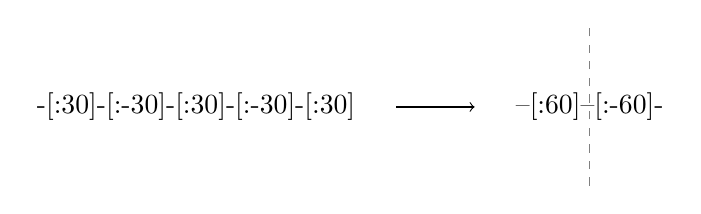
\begin{tikzpicture}
                \node (1) {\chemfig{-[:30]-[:-30]-[:30]-[:-30]-[:30]}};
                \node (2) at (5,0) {\chemfig{--[:60]--[:-60]-}}
                    edge [<-,shorten <=4mm,shorten >=4mm] (1)
                ;
        
                \draw [gray,dashed] (5,-1) -- ++(0,2);
            \end{tikzpicture}
            \caption{Mirror plane in hexane.}
            \label{fig:hexaneMirrorPlane}
        \end{figure}
        \item No symmetry, such as in 1-bromo-2,5-dichloro-3,4,6-trimethylbenzene, means all (nine) distinct signals.
        \item Local symmetry (think an isopropyl group).
        \begin{itemize}
            \item Look for branch points.
            \item You must have consistency of structure for the entirety of branches.
        \end{itemize}
        \item para-dibromobenzene has only 2 signals since it has \emph{two} mirror planes.
    \end{itemize}
\end{itemize}



\section{NMR}
\begin{itemize}
    \item \marginnote{1/13:}He is going to try and present a different perspective from the book because otherwise, why take the class.
    \item There is no preset curve for this class --- everyone can get an A.
    \item The right and left boards will be there for the whole class, every class.
    \item \ce{H3O+} workup.
    \begin{figure}[h!]
        \centering
        \footnotesize
        \schemestart
            \chemfig{=_[:30]-[:-30]-[:30]=^[2]O}
            \arrow{->[\ce{Nu-}]}
            \chemleft{[}
                \chemfig{=_[:30]-[:-30]-[:30](-[2]\charge{45:3pt=$\ominus$}{O})(-[:-30]Nu)}
            \chemright{]^-}
            \arrow{->[\ce{H3O+}][workup]}[,1.2]
            \chemfig{=_[:30]-[:-30]-[:30](-[2]OH)(-[:-30]Nu)}
        \schemestop
        \caption{\ce{H3O+} workup.}
        \label{fig:H3Oworkup}
    \end{figure}
    \begin{itemize}
        \item Don't think acid-catalyzed hydration. Acid-catalyzed hydration is a very specific reaction. Organic chemists don't really use it because those conditions are so acidic that no other functional groups survive it.
        \item An \ce{H3O+} workup is adding \ce{H3O+} at the end of a reaction to neutralize the structure and excess nucleophile in solution without affecting other groups.
    \end{itemize}
    \item Next three lectures: Tools for characterizing molecules, e.g., determining what we have in solution.
    \item It could take decades or even centuries to determine the structure of molecules in the early days of chemistry.
    \begin{itemize}
        \item It would also take large quantites for experiments.
        \item Now we can determine the structures of quantities we can only isolate milligrams of.
    \end{itemize}
    \item IR can only identify the presence of some functional groups and maybe the identity of a compound that's already been determined (i.e., from the fingerprint region and an online database).
    \item NMR.
    \begin{itemize}
        \item Such machines exist in hospitals as MRI.
        \item We have dropped the "N" in NMRI because of nuclear's negative connotation, even though MRI machines have nothing to do with radioactivity.
    \end{itemize}
    \item Any nucleus that has an odd atomic number will have a dipole moment.
    \begin{itemize}
        \item The four most significant ones for organic chemistry are \ce{{}^1H}, \ce{{}^13C}, \ce{{}^15N}, and \ce{{}^17O}.
        \item The last three are all not commonly occurring isotopes. Oxygen, especially, can barely be measured. Hydrogen will be the most useful because \ce{{}^1H} is the most commonly occurring isotope.
        \item For \ce{{}^13C}, we will need a longer experiment since only 1/1000 carbon atoms is \ce{{}^13C}.
    \end{itemize}
    \item Theory-lite for NMR.
    \begin{itemize}
        \item Parallel spins are lower energy, but the difference in energy from anti-parallel is very small (approximately $\SI[per-mode=symbol]{5e-6}{\kilo\calorie\per\mole}$).
        \item $\SIrange{1}{20}{\milli\gram}$ of compound is needed in $\SI{0.75}{\milli\liter}$ of solvent.
        \item This is a non-destructive process --- we can recover our compound after running the experiment.
        \item We typically use \ce{CDCl3} as our solvent.
        \item A part per million (ppm) is a Hz/MHz.
    \end{itemize}
    \item George Van Dyke Tiers, a grad student at UChicago, determined in 1958 that TMS might be the best standard (low chemical shift, chemically inert, easily removed, etc.).
    \item Goes over examples from office hours.
    \item DEPT: Changes the angle of the magnetic field to distinguish \ce{CH}, \ce{CH2}, and \ce{CH3} groups.
    \begin{itemize}
        \item DEPT 90 changes the angle by $\ang{90}$; DEPT 135 by $\ang{135}$.
        \item In DEPT 90, we'll only see \ce{CH} carbons.
        \item In DEPT 135, \ce{CH} and \ce{CH3} groups will peak in the positive direction, and \ce{CH2} groups will peak in the negative direction.
        \item Neither experiment will show carbons that aren't bonded to any hydrogens.
        \item Note that DEPT works for any type of carbon of any hybridization; it only discriminates based on the number of \ce{{}^1H}'s attached.
    \end{itemize}
\end{itemize}



\section{Chapter 9: Nuclear Magnetic Resonance and Mass Spectroscopy}
\emph{From \textcite{bib:SolomonsEtAl}.}
\begin{itemize}
    \item \marginnote{1/11:}\textbf{Nuclear magnetic resonance spectrum}: A graph that shows the characteristic energy absorption frequencies and intensities for a sample in a magnetic field. \emph{Also known as} \textbf{NMR spectrum}.
    \item The chemical shift of a signal gives important clues about molecular structure (see Table \ref{tab:protonChemicalShifts}).
    \begin{table}[H]
        \centering
        \small
        \renewcommand{\arraystretch}{1.4}
        \begin{tabular}{|lc|lc|}
            \hline
            \rule{0pt}{2em}\textbf{Type of Proton} & \textbf{\shortstack{Chemical Shift\\($\bm{\delta}$, ppm)}} & \textbf{Type of Proton} & \textbf{\shortstack{Chemical Shift\\($\bm{\delta}$, ppm)}}\\
            $\ang{1}$ Alkyl, {\sf\ce{RC{\color{rex}H}3}} & \numrange{0.8}{1.2} & Alkyl bromide, {\sf\ce{RC{\color{rex}H}2}Br} & \numrange{3.4}{3.6}\\
            $\ang{2}$ Alkyl, {\sf\ce{RC{\color{rex}H}2R}} & \numrange{1.2}{1.5} & Alkyl chloride, {\sf\ce{RC{\color{rex}H}2}Cl} & \numrange{3.6}{3.8}\\
            $\ang{3}$ Alkyl, {\sf\ce{R3C{\color{rex}H}}} & \numrange{1.4}{1.8} & Vinylic, {\sf\ce{R2C=C{\color{rex}H}2}} & \numrange{4.6}{5.0}\\
            Allylic, {\sf\ce{R2C=CR-C{\color{rex}H}3}} & \numrange{1.6}{1.9} & Vinylic, {\sf\ce{R2C=CR{\color{rex}H}}} & \numrange{5.2}{5.7}\\
            Ketone, {\sf\ce{RCOC{\color{rex}H}3}} & \numrange{2.1}{2.6} & Aromatic, {\sf\ce{Ar{\color{rex}H}}} & \numrange{6.0}{8.5}\\
            Benzylic, {\sf\ce{ArC{\color{rex}H}3}} & \numrange{2.2}{2.5} & Aldehyde, {\sf\ce{RCO{\color{rex}H}}} & \numrange{9.5}{10.5}\\
            Acetylenic, {\sf\ce{RC#C{\color{rex}H}}} & \numrange{2.5}{3.1} & Alcohol hydroxyl, {\sf\ce{RO{\color{rex}H}}} & \numrange{0.5}{6.0}\textsuperscript{*}\\
            Alkyl iodide, {\sf\ce{RC{\color{rex}H}2I}} & \numrange{3.1}{3.3} & Amino, {\sf\ce{R-N{\color{rex}H}2}} & \numrange{1.0}{5.0}\textsuperscript{*}\\
            Ether, {\sf\ce{ROC{\color{rex}H}2R}} & \numrange{3.3}{3.9} & Phenolic, {\sf\ce{ArO{\color{rex}H}}} & \numrange{4.5}{7.7}\textsuperscript{*}\\
            Alcohol, {\sf\ce{HOC{\color{rex}H}2R}} & \numrange{3.3}{4.0} & Carboxylic, {\sf\ce{RCOO{\color{rex}H}}} & \numrange{10}{13}\textsuperscript{*}\\
            \hline
            \multicolumn{4}{l}{\footnotesize\textsuperscript{*}The chemical shifts of these protons vary in different solvents and with temperature and concentration.}
        \end{tabular}
        \caption{Approximate proton chemical shifts.}
        \label{tab:protonChemicalShifts}
    \end{table}
    \item "In \ce{{}^13C} NMR spectroscopy, signal area is not relevant in routine analyses" \parencite[396]{bib:SolomonsEtAl}.
    \item \textbf{Coupling}: The magnetic effect of nonequivalent hydrogen atoms that are within 2 or 3 bonds of the hydrogens producing the signal that splits individual \textbf{signals} into multiple \textbf{peaks}. \emph{Also known as} \textbf{signal splitting}, \textbf{signal multiplicity}.
    \item \textbf{Vicinal} (hydrogens): Hydrogens on adjacent carbons.
    \item \textbf{Geminal} (hydrogens): Hydrogens bonded to the same carbon.
    \begin{itemize}
        \item Coupling occurs between geminal hydrogens in chiral/conformationally restricted molecules, specifically diastereotopic hydrogens.
    \end{itemize}
    \item Interpreting NMR spectra:
    \begin{enumerate}
        \item Count the number of signals in the spectrum to determine how many distinct proton environments there are in the molecule.
        \item Use chemical shift tables (such as Table \ref{tab:protonChemicalShifts}) to correlate the chemical shifts of the signals with possible structural environments.
        \item Determine the relative area of each signal, as compared with the area of other signals, as an indication of the relative number of protons producing the signal.
        \item Interpret the splitting pattern for each signal to determine how many hydrogen atoms are present on carbon atoms adjacent to those producing the signal and sketch possible molecular fragments.
        \item Join the fragments to make a molecule in a fashion that is consistent with the data.
    \end{enumerate}
    \item The external magnetic field causes the $\sigma$ (and $\pi$, if applicable) electrons in the viscinity of each proton to circulate, producing a small local magnetic field that can serve to either increase or decrease the external magnetic field experienced by the proton.
    \begin{itemize}
        \item Increasing the effective field causes a larger chemical shift (it takes a higher energy photon/less magnetic field to induce a spin flip).
        \item Decreasing the effective field causes a smaller chemical shift (it takes less energy/more magnetic field to induce a spin flip).
    \end{itemize}
    \item \textbf{Shielded} (proton): A proton for which the induced local magnetic field opposes the external magnetic field to a relatively large degree. 
    \item \textbf{Deshielded} (proton): A proton for which the induced local magnetic field opposes the external magnetic field to a relatively small degree (or even reinforces the external magnetic field).
    \begin{itemize}
        \item For example, the $\pi$ electrons of benzene circulate in such a way that the external magnetic field at the aromatic hydrogens is \emph{augmented}.
    \end{itemize}
    \item "Chemically equivalent protons are chemical shift equivalent in \ce{{}^1H} NMR spectra" \parencite[403]{bib:SolomonsEtAl}.
    \item \textbf{Homotopic} (atoms): A set of atoms on some molecule such that replacing different ones with the same group gives the same compound.
    \begin{itemize}
        \item For example, the six hydrogens of ethane are homotopic since replacing any of them with chlorine (for instance) gives the same compound: chloroethane.
        \item Homotopic hydrogens are chemical shift equivalent.
    \end{itemize}
    \item \textbf{Heterotopic} (atoms): A set of atoms on some molecule such that replacing different ones with the same group gives different compounds.
    \begin{itemize}
        \item For example, in chloroethane, the \ce{CH2} hydrogens are heterotopic to the \ce{CH3} hydrogens since replacing the former yields 1,1-dichloroethane and replacing the latter yields 1,2-dichloroethane.
        \item Heterotopic atoms are \emph{not} chemical shift equivalent.
    \end{itemize}
    \item \textbf{Enantiotopic} (atoms): Two atoms on some molecule such that replacing different atoms with the same group gives enantiomers.
    \begin{itemize}
        \item Example: The \ce{CH2} hydrogens of bromoethane.
        \item Enantiotopic atoms are chemical shift equivalent, except possibly when the compound in question is dissolved in a chiral solvent.
    \end{itemize}
    \item \textbf{Diastereotopic} (atoms): Two atoms on some molecule such that replacing different atoms with the same group gives diastereomers.
    \begin{itemize}
        \item Example: The \ce{CH2} hydrogens of 2-butanol.
        \item Diastereotopic atoms are \emph{not} chemical shift equivalent (the asymmetry of the chirality center ensures this), except possibly by coincidence.
    \end{itemize}
    \item \textbf{Coupling constant}: The separation in hertz between each peak of a signal. \emph{Denoted by} $\bm{J}$.
    \begin{itemize}
        \item On the order of $\SIrange{6}{8}{\hertz}$.
    \end{itemize}
    \item The reciprocity of coupling constants: The coupling constants of coupled atoms are the same.
    \begin{itemize}
        \item In more complicated molecules, noting that two signals have the same coupling constant means the protons to which they correspond are likely coupled.
    \end{itemize}
    \item \textbf{Dihedral angle} (between vicinal groups): The angle between viscinal groups as seen on the Newman projection through the bond connecting their parent atoms. \emph{Denoted by} $\bm{\phi}$.
    \item \textbf{Karplus correlation}: The dependence of the coupling constant on dihedral angles.
    \begin{itemize}
        \item Discovered by Martin Karplus of Harvard.
        \item Useful for identifying cyclohexane conformations, and thus for determining which conformation is lower energy.
    \end{itemize}
    \item An NMR spectrometer is a camera with a relatively slow shutter speed, in that it blurs pictures of rapidly occurring molecular processes.
    \item Examples of rapid processes that occur in organic molecules.
    \begin{itemize}
        \item Chemical exchanges cause spin decoupling.
        \begin{itemize}
            \item Consider ethanol.
            \item Based on its structure, we'd predict that the signal corresponding to the hydroxyl proton would be a triplet.
            \item However, it only appears as a triplet in very pure ethanol, where \textbf{chemical exchange} is slower due to the reduction in impurity-assisted chemical exchange catalysis common in normal ethanol.
            \item Rapid chemical exchange means that neighboring protons don't have enough time to couple; thus, the hydroxyl proton appears as a singlet in relatively impure ethanol.
            \item Occurs in the \ce{{}^1H} NMR spectra of alcohols, amines, and carboxylic acids; the signals of \ce{OH} and \ce{NH} protons are normally unsplit and broad.
            \item "Protons that undergo rapid chemical exchange\dots can be easily detected by placing the compound in \ce{D2O}. The protons are rapidly replaced by deuterons, and the proton signal disappears from the spectrum" \parencite[413]{bib:SolomonsEtAl}.
        \end{itemize}
        \item Conformational changes.
        \begin{itemize}
            \item If, for example, we could isolate staggered bromoethane, the \ce{CH3} hydrogens would be split into two signals, as the one anti-periplanar hydrogen is in a different chemical environment from its two geminal neighbors.
            \item But we can't, so all three \ce{CH3} hydrogens contribute to one peak.
        \end{itemize}
    \end{itemize}
    \item \textbf{Chemical exchange}: The swapping of identical atoms between molecules.
    \item \textbf{Exchangeable proton}: A proton that can engage in rapid chemical exchange.
    \item We now switch gears to \ce{{}^13C} NMR spectroscopy.
    \item Although \ce{{}^13C} does not occur naturally with nearly the same frequency as \ce{{}^12C}, it is important for its application to NMR spectroscopy.
    \item Simplifications from \ce{{}^1H} NMR spectroscopy.
    \begin{itemize}
        \item Each distinct carbon produces one signal in a \ce{{}^13C} NMR spectrum.
        \item Splitting of \ce{{}^13C} signals into multiple peaks is not observed in routine \ce{{}^13C} NMR spectra.
    \end{itemize}
    \item No (technically just very little) carbon-carbon coupling since coupling only occurs for adjacent carbons and only 1 in 100 carbon atoms is \ce{{}^13C} ($\SI{1.1}{\percent}$ natural abundance).
    \item Carbon-proton coupling can occur, however, splitting \ce{{}^13C} signals into multiplets.
    \item \textbf{Broadband proton decoupled} (spectrum): A \ce{{}^13C} NMR spectrum in which \ce{{}^1H}-\ce{{}^13C} coupling is eliminated by choosing instrumental parameters to decouple the proton-carbon interactions. \emph{Also known as} \textbf{BB proton decoupled}.
    \item Shielding and deshielding works the same way (see Table \ref{tab:carbonChemicalShifts}).
    \begin{table}[H]
        \centering
        \small
        \renewcommand{\arraystretch}{1.4}
        \begin{tabular}{|lc|}
            \hline
            \rule{0pt}{2em}\textbf{Type of Carbon} & \textbf{\shortstack{Chemical Shift\\($\bm{\delta}$, ppm)}}\\
            $\ang{1}$ Alkyl, {\sf\ce{R{\color{rex}C}H3}} & \numrange{0}{40}\\
            $\ang{2}$ Alkyl, {\sf\ce{R{\color{rex}C}H2R}} & \numrange{10}{50}\\
            $\ang{3}$ Alkyl, {\sf\ce{R{\color{rex}C}HR2}} & \numrange{15}{50}\\
            Alkyl halide or amine, {\sf\ce{R3{\color{rex}C}X}} ($\ce{X}=\ce{Cl},\ce{Br},\ce{NR$'$2}$) & \numrange{10}{65}\\
            Alcohol or ether, {\sf\ce{R3{\color{rex}C}OR$'$}} & \numrange{50}{90}\\
            Alkyne, {\sf\ce{R{\color{rex}C}#R$'$}} & \numrange{60}{90}\\
            Alkene, {\sf\ce{R2{\color{rex}C}=R$'$}} & \numrange{100}{170}\\
            Aryl, {\renewcommand*\printatom[1]{\ensuremath{\mathsf{#1}}}\chemfig[atom sep=1.4em]{[:30]**6(--{\color{rex}C}(-R)----)}} & \numrange{100}{170}\\
            Nitrile, {\sf\ce{R{\color{rex}C}#N}} & \numrange{120}{130}\\
            Amide, {\sf\ce{R{\color{rex}C}ONR$'$2}} & \numrange{150}{180}\\
            Carboxylic acid or ester, {\sf\ce{R{\color{rex}C}OOR$'$}} & \numrange{160}{185}\\
            Aldehyde or ketone, {\sf\ce{R{\color{rex}C}OR$'$}} & \numrange{182}{215}\\
            \hline
        \end{tabular}
        \caption{Approximate carbon-13 chemical shifts.}
        \label{tab:carbonChemicalShifts}
    \end{table}
    \item In addition to the TMS peak, \ce{{}^13C} spectra have a \ce{CDCl3} solvent peak at $\delta\ 77$.
    \item \textbf{DEPT \ce{{}^13C} NMR spectrum}: A \ce{{}^13C} NMR spectrum that indicates how many hydrogen atoms are bonded to each carbon, while also providing the chemical shift information contained in a broadband proton-decoupled \ce{{}^13C} NMR spectrum. \emph{Also known as} \textbf{distortionless enhancement by polarization transfer}.
\end{itemize}




\end{document}